\documentclass[10pt,a4paper,twoside]{article}
\usepackage[a4paper,top=20mm,bottom=20mm,outer=5cm]{geometry}
\usepackage[utf8]{inputenc}
\usepackage[english]{babel}
\usepackage{graphicx}
\usepackage{hyperref}
\usepackage{amsmath}
\usepackage{listings}
\usepackage{cleveref}
\usepackage{natbib}
\bibliographystyle{abbrvnat}
\setcitestyle{authoryear}

\title{Project Machine Learning\\--- Milestone 1 ---} 

%%%%%%%%%%%%%%%%%%%%%%%%%%%%%%%%%%%%%%%
%                                     %
%   EVERYTHING BELOW CAN BE CHANGED   %
%                                     %
%%%%%%%%%%%%%%%%%%%%%%%%%%%%%%%%%%%%%%%

\author{Konstantin Ausborn, Timon Palm, Marco Rosinus Serrano}
\date{\today}

\begin{document}
\maketitle

\section{Introduction}
In the course of this machine learning project, we aim to implement a Vector-Quantized Variational Autoencoder (VQ-VAE) \cite{vqvae} and to reproduce their results on the ImageNet and CIFAR-10 datasets.

In the first milestone, we focus on data preprocessing and the implementation of a baseline method for subsequent comparison. This section will provide an overview of the datasets we will use, the preprocessing steps applied, and the baseline method we will implement. Additionally, we will outline the evaluation metrics that will be used to compare the performance of our VQ-VAE model with the baseline method.

Upon examining the ImageNet dataset, we found that it contains images with highly irregular resolutions, including some very small images, which was unexpected. As a result, we performed additional data cleaning by removing images that were excessively small.

\section{Dataset overview}
    Vector-quantized variational autoencoders (VQ-VAE) are versatile models that can be applied to various modalities, including image, video, and audio generation. In this project, we will primarily focus on image generation, drawing comparisons with earlier models such as the classic Autoencoder and Variational Autoencoder (VAE) \cite{vae}.

    The original VQ-VAE paper \cite{vqvae} trained their model on three image datasets: \textit{ImageNet}, \textit{CIFAR-10}, and video frames from \textit{DeepMind Lab}. For this project, we will follow the same approach and train our VQ-VAE model on the ImageNet and CIFAR-10 datasets.

    Image generation is an unsupervised learning task and therefore does not require labeled data. Potentially, any kind of image data could be used for training and testing. However, the quality of the generated images is highly dependent on the quality and diversity of the training data.

    Further feature extraction methods are not necessary for the image generation task, as VQ-VAE works directly on pixel values. Image pixels are numerical values with a spatial correlation that VQ-VAE leverege. VQ-VAE follows the Encoder-Decoder structure, learning a compressed representation of the input image in latent space. Thus, VQ-VAE itself can be seen as a feature extraction/compression method.

    ImageNet and CIFAR-10 are among the most common image datasets used in machine learning. While they were originally designed for image classification and detection tasks, their utility extends beyond these applications; by discarding the labels, they can also be leveraged for image generation tasks. An overview of these two datasets is provided in Table \ref{tab:datasets}
    
    \subsection{ImageNet}
    The full ImageNet dataset consists of 14.197.122 hand-labeled photographs collected from flickr and other search engines \cite{ILSVRC15}\cite{imagenet_breakdown}. The images are distributed over 21841 \textit{synonym sets} from the \textit{WordNet} \cite{wordnet} hierarchy, pursuing to cover most nouns in the English language \cite{imagenet_breakdown}.

    When talking about ImageNet, most authors refer to the \textit{ImageNet Large Scale Visual Recognition Challenge 2012} (ILSVRC) dataset \cite{ILSVRC15}, which is a subset of the full dataset. Hereinafter, we will refer to the ILSVRC 2012 dataset as ImageNet if not stated otherwise.
    
    The ILSVRC set contains 1.281.167 unique labeled training images and 100.000 labeled test images distributed over 1000 classes.
     
    ILSVRC was created as a computer vision benchmark. It therefore additionally contains 50.000 validation images without labels, which we will not consider.
    Three key computer vision tasks are benchmarked by the ILSVRC dataset: object classification, object localization and object detection.
    They address three fundamental computer vision questions: \textit{What is in the image?}, \textit{Where is it?} and \textit{How many are there?}.

    ImageNet is a supervised learning dataset with class id and bounding box annotations. Though, it can also be used for unsupervised learning tasks like image generation, image compression or image denoising.
    
    The collected images neither contain missing values nor duplicates and every image belongs to exactly one class.

    The ImageNet dataset is designed to capture a diverse range of real-world scenarios across eight dimensions, as illustrated in Figure \ref{fig:imnet_dimensions} from \cite{imagenet_breakdown}. These dimensions include object scale (ranging from small to large objects), the number of instances (from few to many objects present in an image), as well as variations in color and shape distinctiveness.

   \begin{figure}
        \centering
        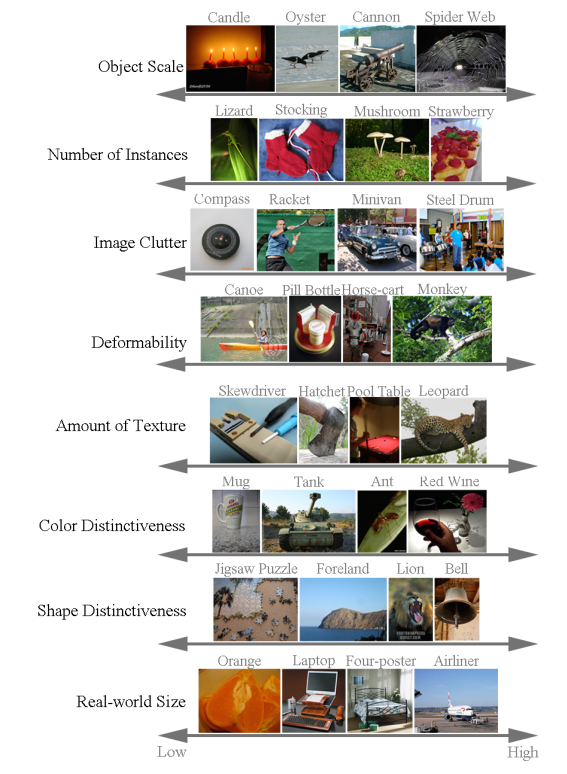
\includegraphics[width=\textwidth]{../../sample_images/imnet_dimension.png}
        \caption{Eight diversity dimensions of the ImageNet dataset \cite{imagenet_breakdown}}
        \label{fig:imnet_dimensions}
   \end{figure}

    The majority of classes contain 1300 examples, though it is not entirely balanced across the classes. In fact, some classes have fewer examples, as shown in Figure \ref{fig:imnet_dist}. Among the classes with the lowest number of images are \textit{"black-and-tan coonhound"}, \textit{"otterhound"} and \textit{"English foxhound"} with 732, 738 and 754 samples, respectively. Note: These are different dog breeds

    A class disbalance in the training data can lead to a bias in the resulting model. We access the class distribution in the ImageNet dataset more or less balanced, as most classes contain 1300 images. The classes with fewer examples are still represented by a reasonable number of images. Moreover, the number samples for different dog breeds for instance might be lower, but still the number of dog images is fairly high. Our goal for this project might not be to generate images of different dog breeds, just a dog image suffices.

    Upon examining the plethora of different shapes present in the ImageNet dataset, we found that the images have highly irregular resolutions. The resolutions range from 8x10 pixels to 9331x6530 pixels with a mean resolution of 471.7x404.7 pixels, as shown in Figure \ref{fig:imnet_sizes_err}. The histogram in Figure \ref{fig:imnet_sizes_hist} illustrates the distribution of image resolutions in the dataset.

    As to be seen in figure \ref{fig:optimal_resolution}, some images have a very unregular ratio, which imposes a challenge for resizing. Very small images do not contain enough information, which when upscaled, result in a blurry image (illustrated in figure \ref{fig:small_image}). We decided to remove such images and resstrict the dataset to a minimum image size of 32x32 pixels.

    \begin{figure}
        \centering
        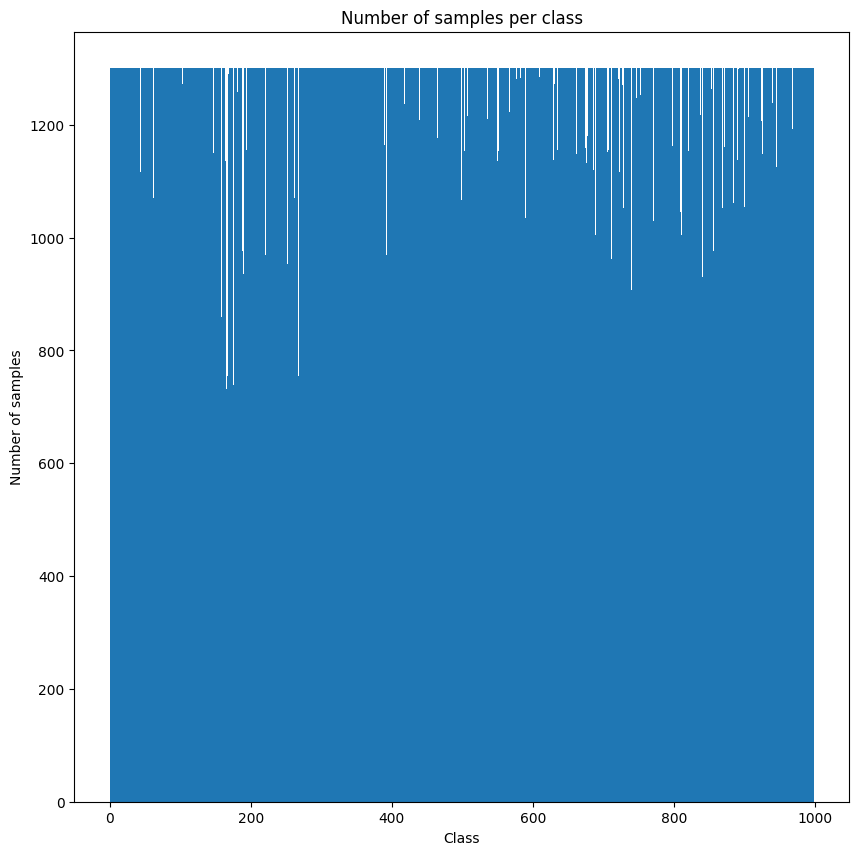
\includegraphics[width=\textwidth]{../../sample_images/imagenet_dist.png}
        \caption{Distribution of images per class in the ImageNet dataset}
        \label{fig:imnet_dist}
    \end{figure}

    \subsubsection{Preprocessing}
    In order to train the VQ-VAE on the ImageNet dataset, we will do the following preprocessing steps.

    \begin{itemize}
        \item \textbf{Image Resizing:} For training and testing, we resize all images to 128x128 pixels, similar to the paper \cite{vqvae}. By virtue of the VQ-VAE architecture, a latent space of 32x32x1 pixel is implied.
        There are different ways one can resize an image. We use a composition of random cropping to extract a square image and resize it to 128x128 pixels with the TorchVision \texttt{v2.RandomResizedCrop(size, scale, ratio, antialias=True)}. We set \texttt{scale=(0.2, 1.0)} and \texttt{ratio=1} to crop a square image with a sufficient area in relation to the original image.\\
        We keep the standard \textit{Bilinear interpolation} for resizing and set \texttt{antialias=True} to reduce aliasing artifacts.

        \item \textbf{MinMax Normalizing:} The pixel values of the images are in the range of 0 to 255. We scale them to the range of 0 to 1 by dividing them by 255. When input features have different scales, normalizing is a necessity for stable convergence. In the case of images, the pixel values are already in the same range, but normalizing them will help to stabilize the training process.

        \item \textbf{Standardization:} Standardizing is a common step in machine learning and also often used for ImageNet, e.g. for training ResNet \cite{resnet}. It is also part of the standard TensorFlow and PyTorch preprocessing pipeline for ImageNet. \\
        We standardize the images with the mean $\mu = (0.485, 0.456, 0.406)$ and standard deviation $\sigma = (0.229, 0.224, 0.225)$ of Imageet for the three color channels, respectively.
    
    \end{itemize}

    Example images from ImageNet dataset after preprocessing are depicted in figure \ref{fig:imnet_example_normalized}.

    \subsection{CIFAR-10}
    CIFAR-10 \cite{cifar10} is another popular image classification dataset, as well as the larger version CIFAR-100. CIFAR-10 consists of 60.000 32x32 pixel images, which are distributed over 10 classes. The dataset is split into 50.000 training images and 10.000 test images. The classes are mutually exclusive, so each image belongs to exactly one class. The classes are: \textit{airplane, automobile, bird, cat, deer, dog, frog, horse, ship, truck}

    The train set contains exactly 5000 images per class, while the test set contains 1000 images per class. No image belongs to more than one class and there are no missing values or duplicates in the dataset.

    \subsubsection{Preprocessing}
    As the images in the CIFAR-10 dataset are already 32x32 pixels, we do not need to resize them. Hence, we will only apply MinMax Normalizing and potentially Standardizing, same as for the ImageNet data.

    Example images from the CIFAR-10 dataset are shown in figure \ref{fig:cifar10_example_normalized}.

    \begin{table}[]
        \begin{tabular}{lllll}
        Dataset & \# train images & \# test images & \# classes & image size \\ \hline \hline
          ILSVRC  & 1.281.167    &        100.000        &      1000       &    8-10px - 9331x6530px       \\
        CIFAR-10   &        50.000     &      10.000      &    10    &     32x32px       \\ \hline \hline
        \end{tabular}
        \caption{Datset overview: ImageNet and CIFAR-10}
        \label{tab:datasets}
    \end{table}

\section{Baseline method and evaluation}

\begin{itemize}
    \item basically just use negative log entropy as the factor to compare
    \item this describes the entropy of the picture generated?
    I do not have clarity here see: https://bjlkeng.io/posts/a-note-on-using-log-likelihood-for-generative-models/
    \item I need to understand PixelCNN better to continue
    \item see Shannon for theory on entropy\cite{shannon}
    \item dont use parzen windows\cite{note_on_eval}
    \item
    \item
\end{itemize}

\section{Discussion}
:-)

\bibliography{bibliography}

\section{Appendix}

\begin{figure}
    \centering
    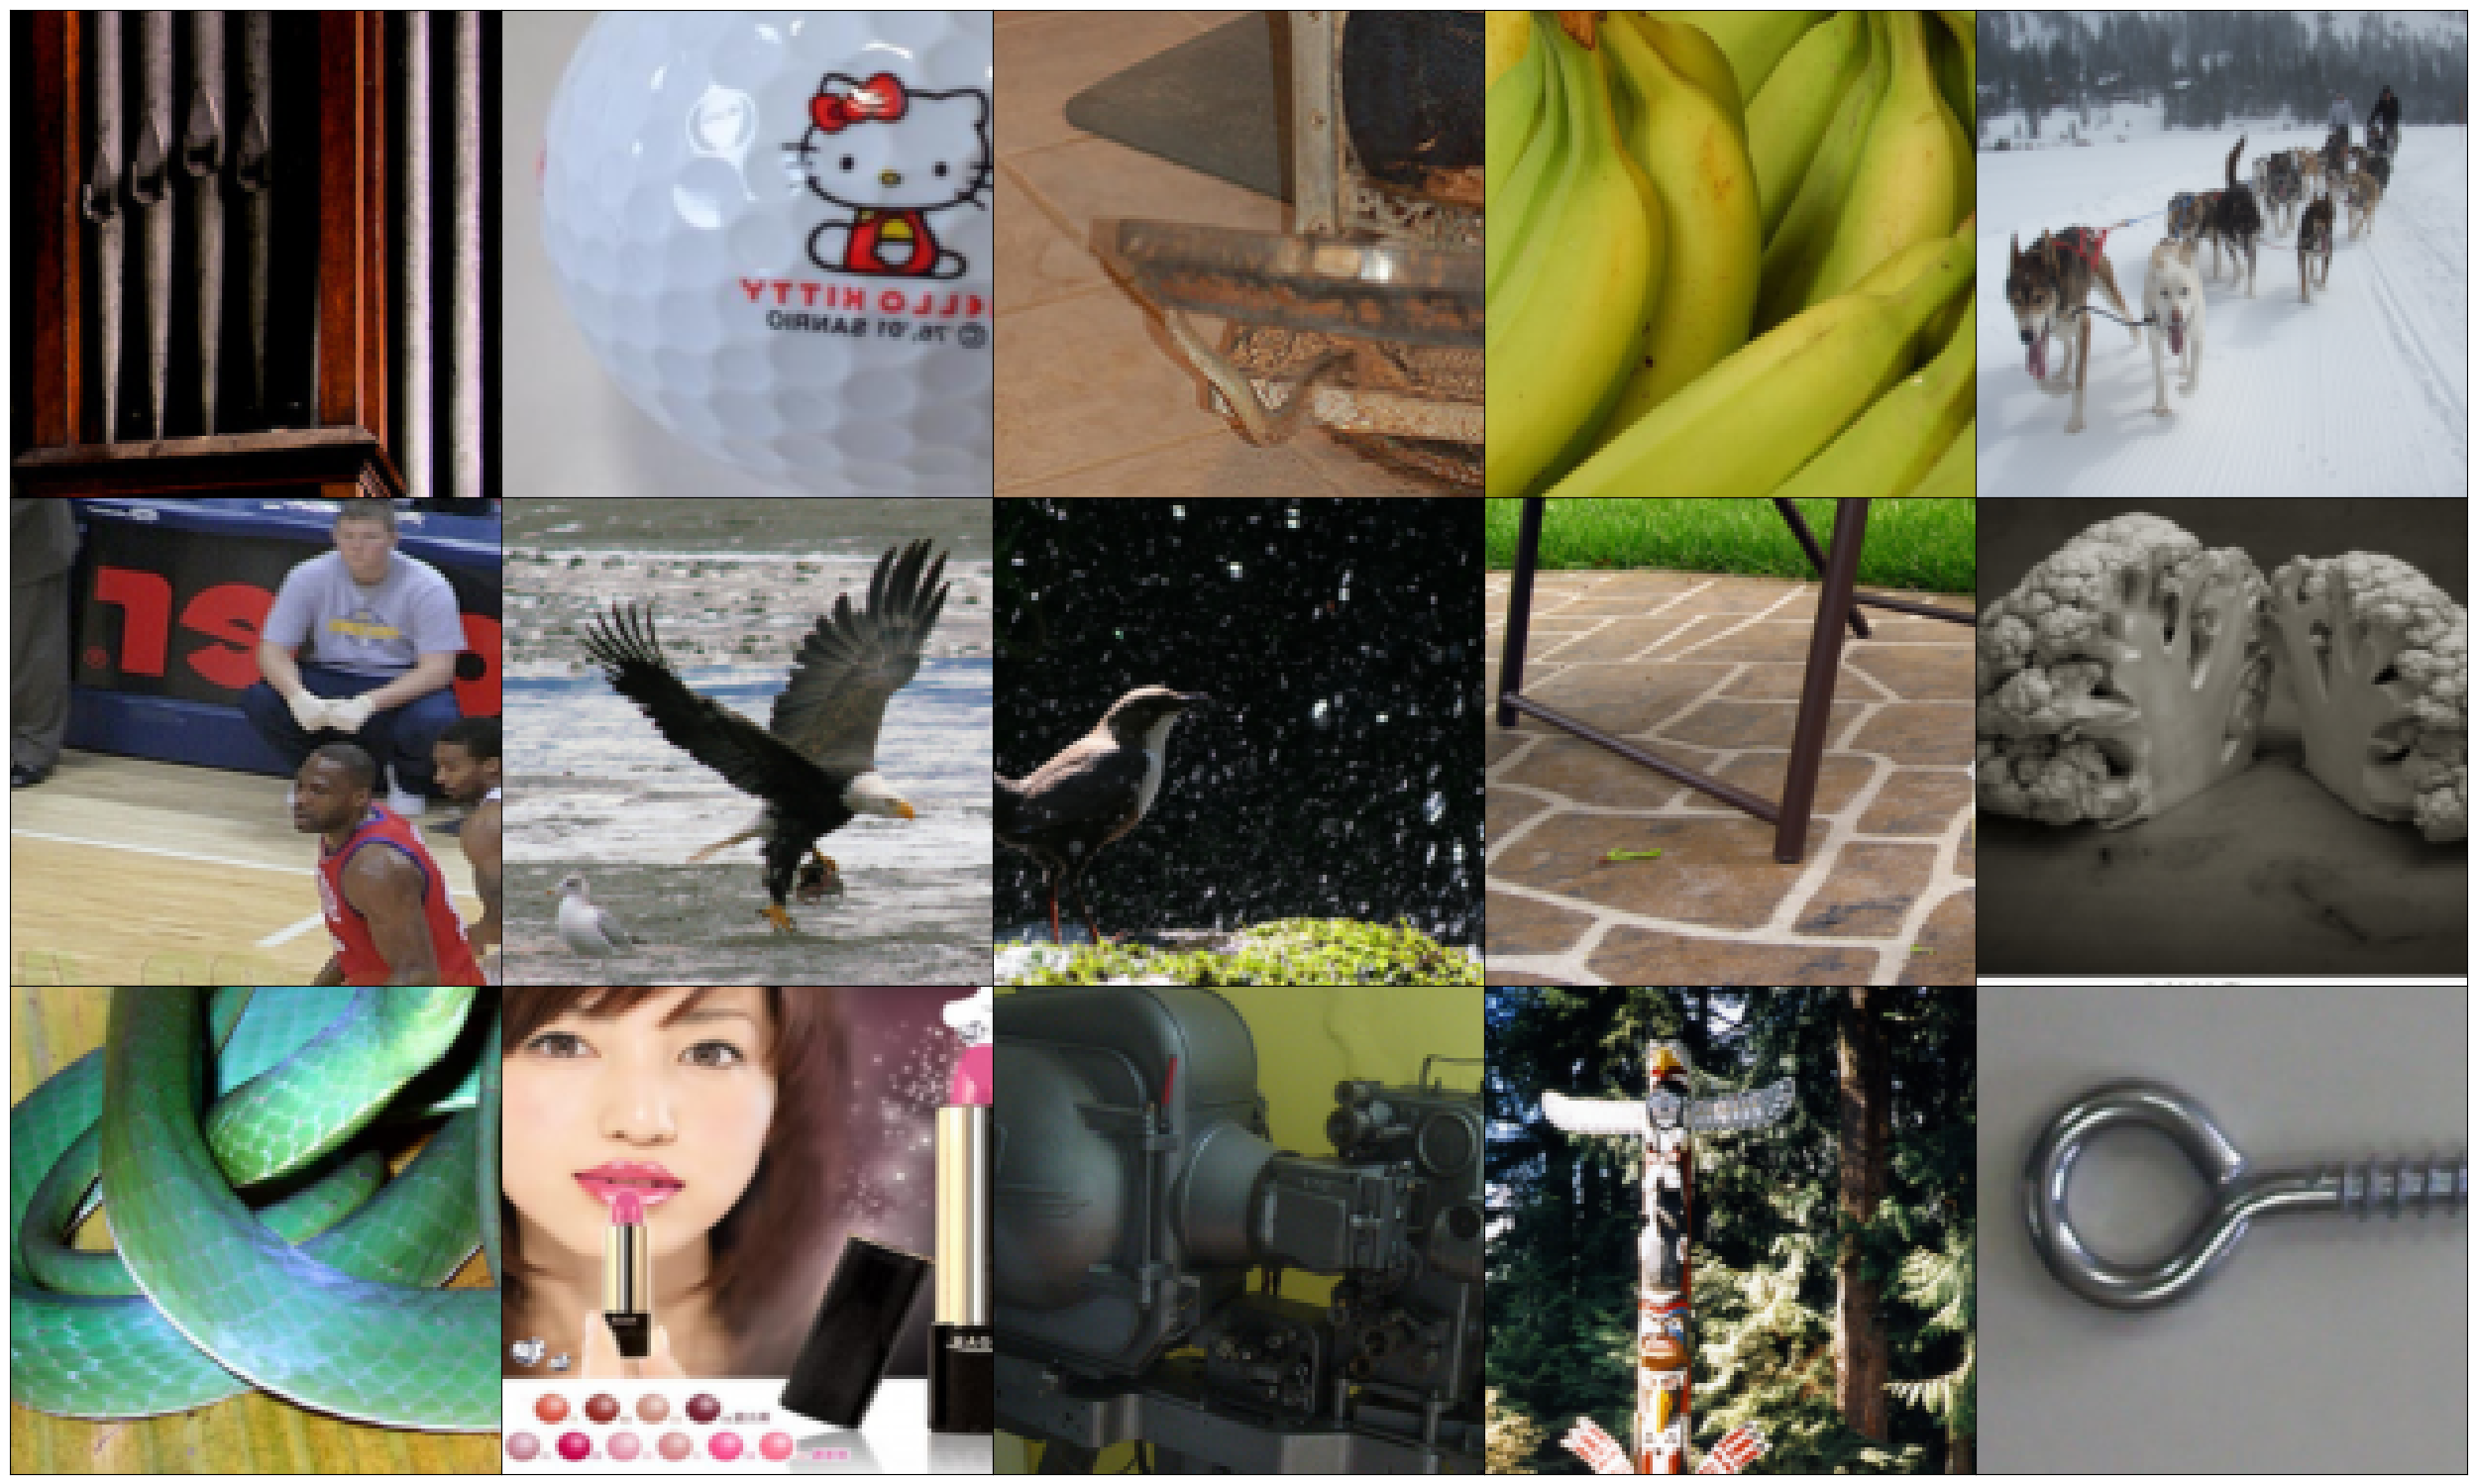
\includegraphics[width=\textwidth]{../../sample_images/imagenet_unnormalized.png}
    \caption{Example images from the ImageNet dataset randomly cropped and resized to 128x128 pixels and standardized}
    \label{fig:imnet_example_normalized}
\end{figure}

\begin{figure}
    \centering
    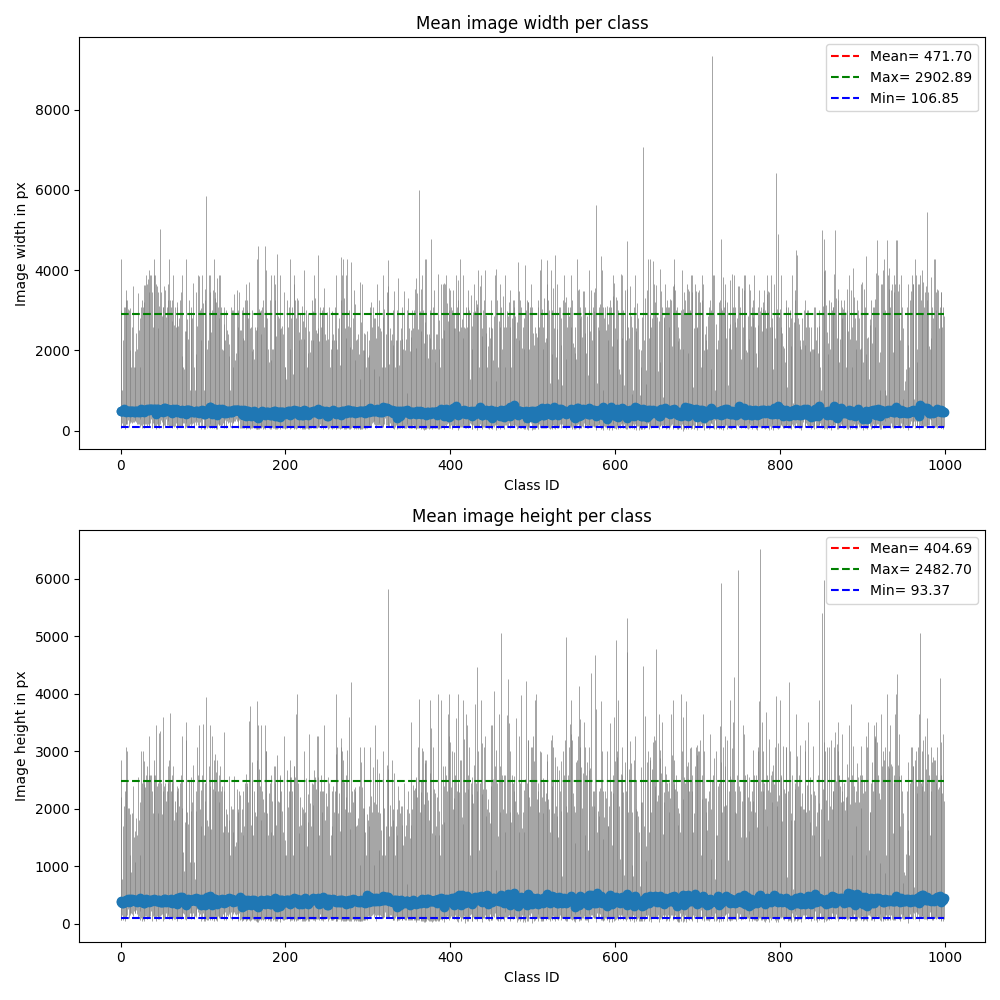
\includegraphics[width=\textwidth]{../../sample_images/imagenet_sizes_errorbar.png}
    \caption{Image resolution deviations in the ImageNet dataset across classes}
    \label{fig:imnet_sizes_err}
\end{figure}

\begin{figure}
    \centering
    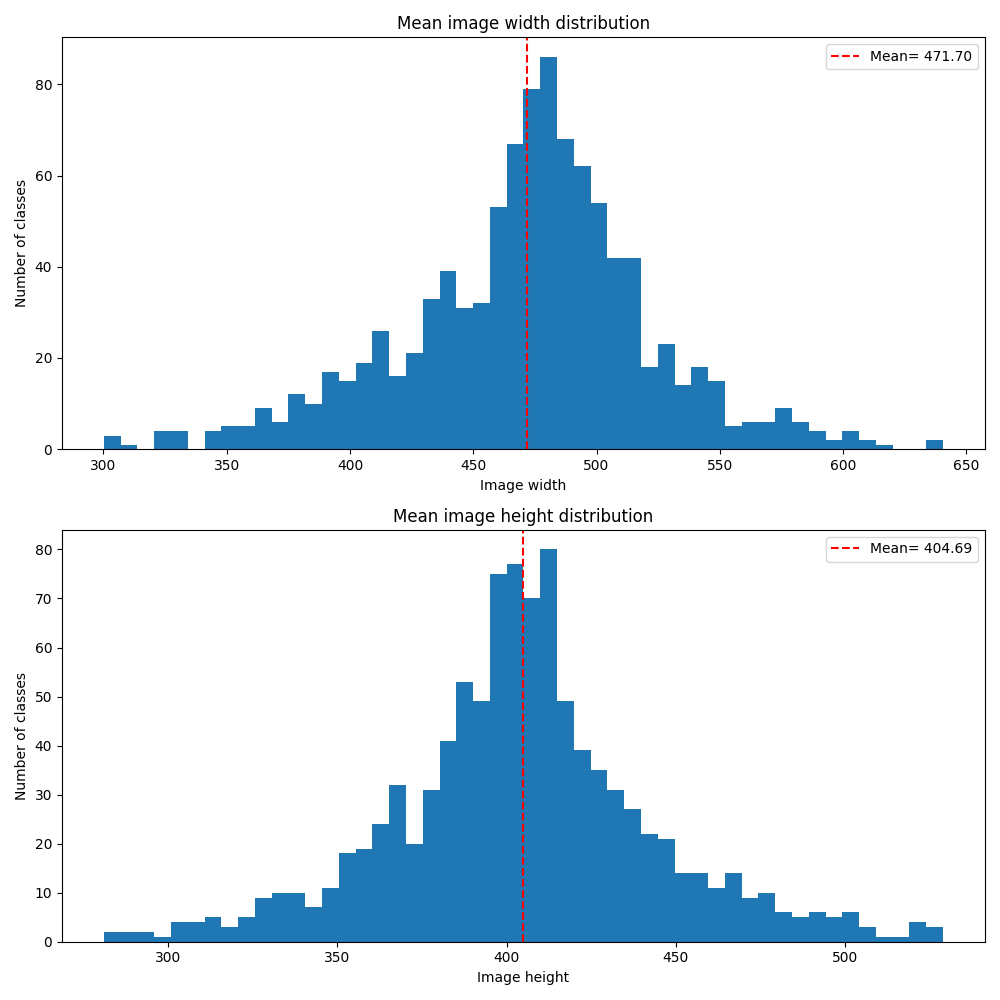
\includegraphics[width=\textwidth]{../../sample_images/imagenet_sizes_histogram.png}
    \caption{Histogram of image resolutions in the ImageNet dataset}
    \label{fig:imnet_sizes_hist}
\end{figure}

\begin{figure}
    \centering
    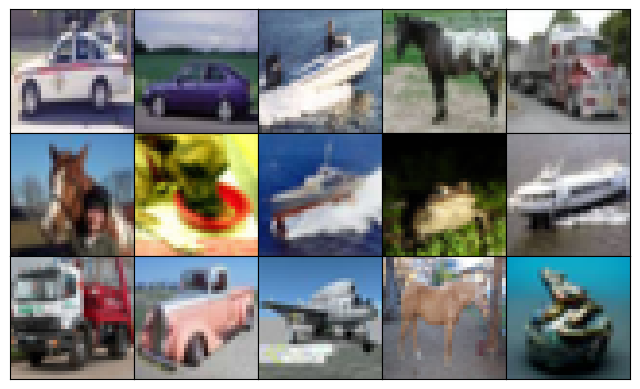
\includegraphics[width=\textwidth]{../../sample_images/cifar_rbatch.png}
    \caption{Example images from the CIFAR-10 dataset standardized}
    \label{fig:cifar10_example_normalized}
\end{figure}

\begin{figure}
    \centering
    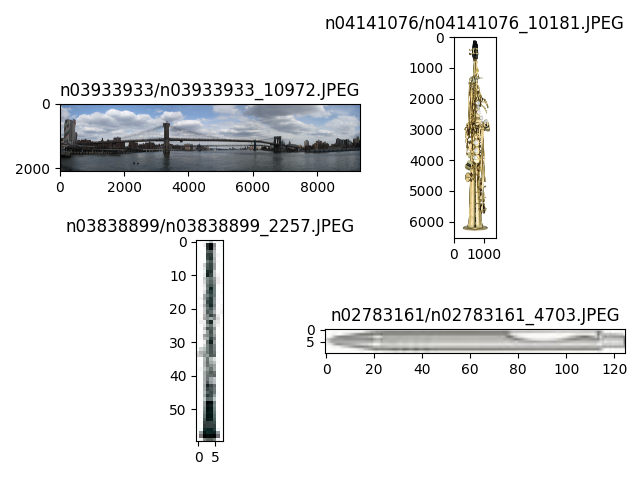
\includegraphics[width=\textwidth]{../../sample_images/optima_shape_examples.png}
    \caption{Example images from the ImageNet dataset with very unregular resolution ratios}
    \label{fig:optimal_resolution}
\end{figure}

\begin{figure}
    \centering
    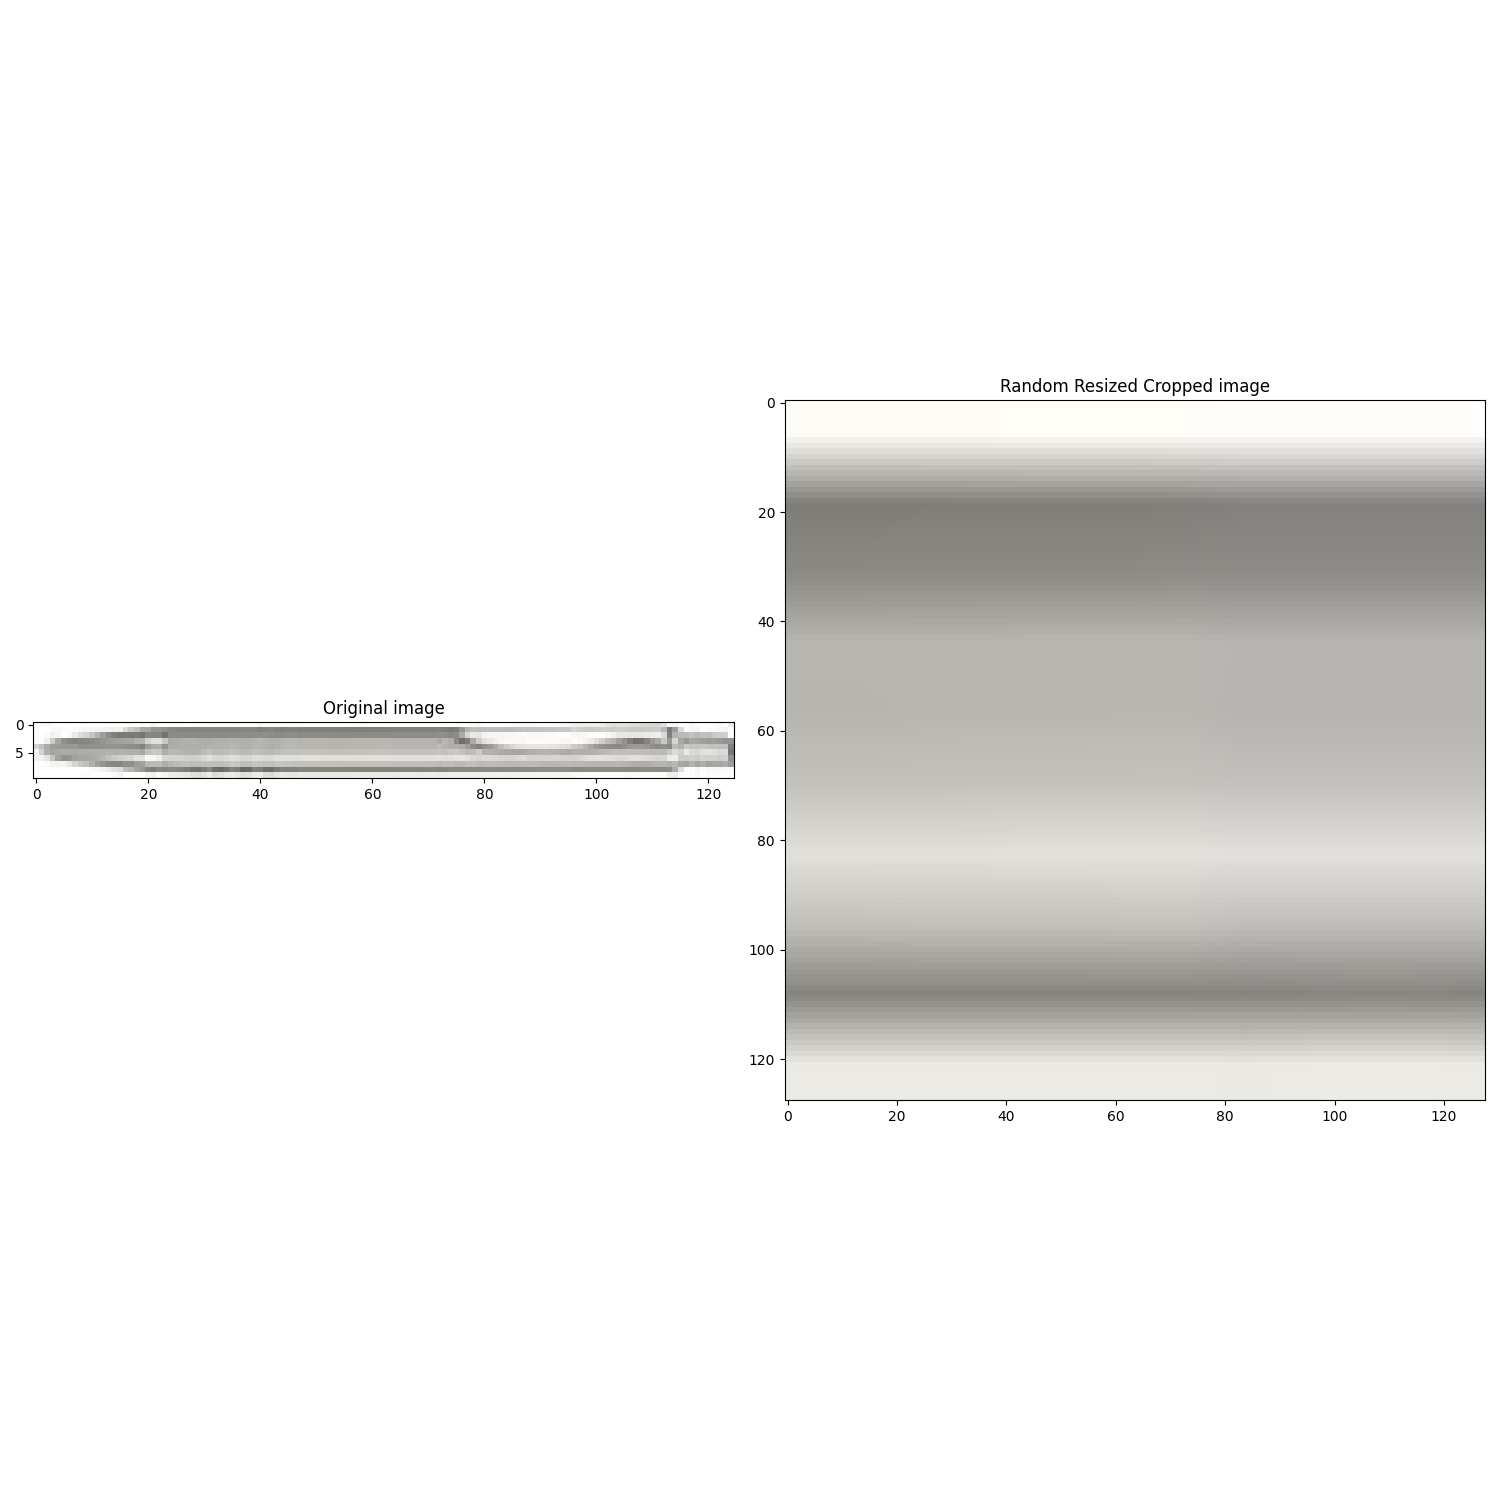
\includegraphics[width=\textwidth]{../../sample_images/random_resized_crop_small.png}
    \caption{Example image from the ImageNet dataset that is too small}
    \label{fig:small_image}
\end{figure}

\end{document}
